\subsection{Heavy Quark-States (b,c)}
Patterns apply here as well. Using the quantum numbers as described in \cref{fig: quark_quantum_numbers}, we can find the quark content of the mesons in \cref{fig: heavy_baryon_nonets}

\begin{figure}[h!]
\centering
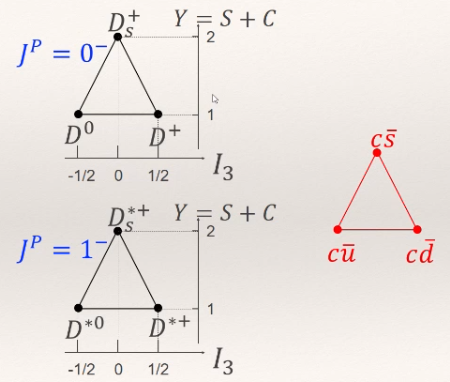
\includegraphics[width = .75\textwidth]{heavy_baryon_nonets.png}
\caption{Caption}
\label{fig: heavy_baryon_nonets}
\end{figure}


\subsubsection{Heavy Quarkonia}
\begin{itemize}
    \item Charmonium $c \bar{c}$ and Bottomonium $b \bar{b}$ are bound states of heavy quarks.
    \item They have the same quantum numbers as the virtual photon if $J^{PC} = 1 ^{--}$
    \item Process is shown in \cref{fig: heavy_quarkonia}
    \item \textbf{OZI rule}: Heavy quarks are suppressed in creatin/annihilation. This means they have long lifetimes. 
    \item For non-$J^{CP} = 1^{- - }$, we can still get heavier quarks, if there is emitted two photons, as they can have different quantum numbers.
    
    \begin{figure}[h!]
    \centering
    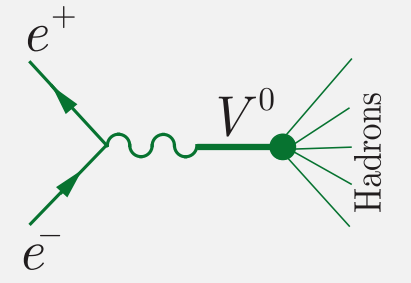
\includegraphics[width = .6\textwidth]{heavy_quarkonia.png}
    \caption{Production of heavy quarkonia in $e^+e^-$ annihilation.}
    \label{fig: heavy_quarkonia}
    \end{figure}
\end{itemize}

\paragraph{Potential:}
\begin{itemize}
    \item It was neither a radial or harmonic oscillator potential that could describe the heavy quarkonia.
    \item The solution was a linear term added to a radial term. This could also be a logarithmic term.
    \item $V(r) = - \frac{a}{r} + br$
    \item This points to a force between the quarks that increases as distance increases.
    \item The mass is then $M(q \bar{q}) = 2m_{q} + E(n,L)$, with $n$ being the principle quantum number.  
    \item The potential is flavour independent. 
\end{itemize}

\subsubsection{Exotic Hadrons}
\begin{itemize}
    \item tetraquarks and pentaquarks, etc. 
    \item Has spin 2. 
\end{itemize}

\section{List of Concepts}
\begin{itemize}
    \item Leptons
    \item Neutrinos
    \item Quarks 
    \item Hadrons 
    \item Lepton universality 
    \item Spectator model 
    \item Yukawa potential
    \item Range of force 
    \item Amplitude 
    \item Resonance
    \item Breit-Wigner distribution 
    \item Lifetime 
    \item Decay rate 
    \item Width 
    \item Neutrino flavour eigenstates 
    \item Neutrino mass eigenstates 
    \item Neutrino mixing 
    \item Neutrino oscillations
    \item Sterile neutrino
    \item Isospin 
    \item Isospin multiplet
    \item Hadron parity 
    \item $Q, B, Y, I, S, C, \tilde{B}, T$
    \item Baryon quark, spin wavefunction 
\end{itemize}


\section{Quark Dynamics: The Strong Interaction}
\subsection{Quantum Chromodynamics (QCD)}
\begin{itemize}
    \item Quantitative theory of strong interactions 
    \item The gluon has zero mass. 
    \item The gluon couples to conserved color charges. 
    \item Static properties of hadrons, like when emitted from a quark are explained. 
    \item Dynamic properties of hadrons, like when scattered are explained.     
    \item Gluons have color charge, and can interact with it self or each other. This gives a three/four-gluon vertex which is not possible with photons.
    \item Bound states of gluons should exist. They are only predicted to exist. 
\end{itemize}

\subsubsection{Color Wavefunction}
\begin{itemize}
    \item By expanding the wavefunction with a color term, we can uphold the Pauli principle
    \begin{equation}
      Ψ = ψ_{\text{space}}  χ_{\text{spin}} χ_{\text{color}}
    \end{equation} 
    \item There are three possible colors, red, green, and blue, each associated with a conserved charge, called color hypercharge $Y^{C}$ and color isospin $I_3^{C}$. This is shown in \cref{fig: color_numbers}. 
    \item The sum of all three colors can bee seen as a white state. If only anti-quarks are present, we can see that as a black state. The net charge is zero either way. 
\end{itemize}

\begin{figure}[h!]
\centering
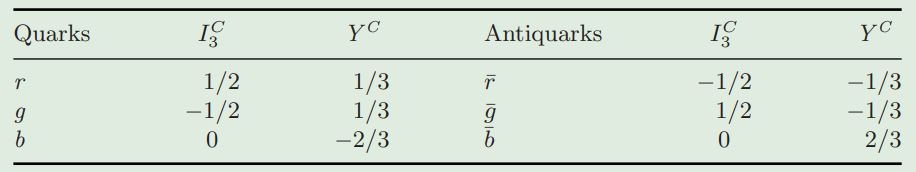
\includegraphics[width = \textwidth]{color_numbers.png}
\caption{Table of quark color and their respective charges. }
\label{fig: color_numbers}
\end{figure}
\subsubsection{Color Confiment}
\begin{itemize}
    \item Hadrons have no net color charge, meaning $I_3^{C} = Y^{C} = 0$. 
    \item The consequence of this is that no long-range gluon mediated strong force happens between nucleons. 
    \item Mesons consist of color-anticolor states. They are therefore "dark". 
    \item Baryons consist of three quarks, and are therefore "white".
    \item The color wavefunction is antisymmetric. 
    \begin{equation}
      χ_{\text{color}} = \frac{1}{\sqrt{6}} \left(r_1g_2b_3 - g_1r_2b_3 - b_1g_2r_3 + g_1b_2r_3 - r_1b_2g_3\right)
    \end{equation}
    \item Allowed numbers of quarks and anti-quarks are $(3q)^{p}(q \bar{q})^{n}$ where $p,n ≥ 0$
    \item Anti-baryons are also allowed, $(3q)^{p}(q \bar{q})^{n} → (3\bar{q})^{l}(3q)^{p}(q \bar{q})^{n}$ where $l,p,n ≥ 0$. 
\end{itemize}



\subsubsection{Gluon Color-States}
\begin{itemize}
    \item The gluon in tasked with keeping the color charge conserved. As seen in \cref{fig: gluon_color_conservation}, the gluon takes the color of the red quark, and passes it on to the blue quark. 
    \item Quarks have only color, but the gluon has color and anti-color. In this case it is $g = r \bar{b}$, as it neutralizes the total color charge and isospin. Summing up the $I_3^{C}$ and $Y^{C}$ of the quarks, gives the remaining value the gluon must have to have net zero charge.
    \item There are only 8 gluons, as the ninth does not interact with the quarks. This is called a non-interacting color singlet. 
\end{itemize}

\begin{figure}[h!]
\centering
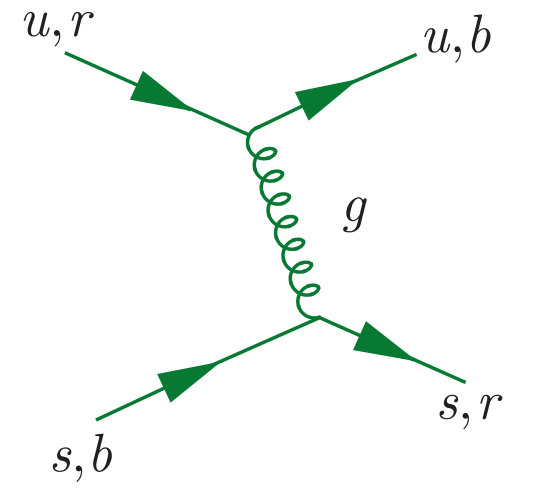
\includegraphics[width = .5\textwidth]{gluon_color_conservation.png}
\caption{Feynman diagram of gluon color conservation.}
\label{fig: gluon_color_conservation}
\end{figure}

\subsubsection{Confinemenet and Hadronization}
\begin{itemize}
    \item At small distances, the quark potential is proportional to $1 / r$. At larger distances, it becomes linear. 
    \item The slope of the linear potential is 1 GeV/fm. This is the same as the mass of the gluon, as the distance between quarks are about 1 fm.
    \item Supplying energy to increase the distance, spawns a jet of new hadrons. 
\end{itemize}

\subsubsection{Confiment and Asymptotic Freedom}
\begin{itemize}
    \item At short distances we have high momentum. Launching a high-energy quark into the hadron lets us look at short-range behavior.
\end{itemize}

\subsection{Running Coupling Constant}
\begin{itemize}
    \item At short distances, the coupling constant becomes small, and 1-gluon exchange is a good model. 
    \item At large distances or low energies, the coupling constant becomes large, and the potential increases with separation. This means gluons are confined inside hadrons. 
    \item The electromagnetic coupling constant increases with higher energies, but the strong coupling constant decreases.
\end{itemize}

\subsubsection{Running $α_s(μ)$ and OZI Rule}   
\begin{itemize}
    \item \textbf{OZI rule}: Creation or annihilation of heavy quarks pairs is suppressed with respect to light quarks. 
    \item Gluons connect the heavy-quark annihilation to the final state of hadrons. 
    \item The running coupling constant leads to reduced gluon coupling to heavy quark pairs, making them suppressed. 
    \item If a quark-antiquark decays, we need more than one gluon to conserve color. As the gluon has the same $C$-parity as the photon ($-1$), we need at least 3 gluons. This leads to suppression. 
\end{itemize}





